\chapter{Motivation}
\label{chapter:introduction}
\section{Problem Statement}
Robot technology is constantly increasing as the performance of the used hardware components enable highly complex software computations. State-of-the-art robots such as REEM-C \cite{reemspec}, Asimo \cite{asimospec}, Hubo \cite{hubospec} and Atlas \cite{atlasspec} indicate that humanoid robots are capable of achieving versatile goals in appropriate time. Videos such as \href{http://www.youtube.com/watch?v=N_m56irWKeI}{this}\footnote{\url{http://www.youtube.com/watch?v=N_m56irWKeI}} expose the remarkable speed of kinematic capabilities.
\begin{figure}[h!]
  \centering
    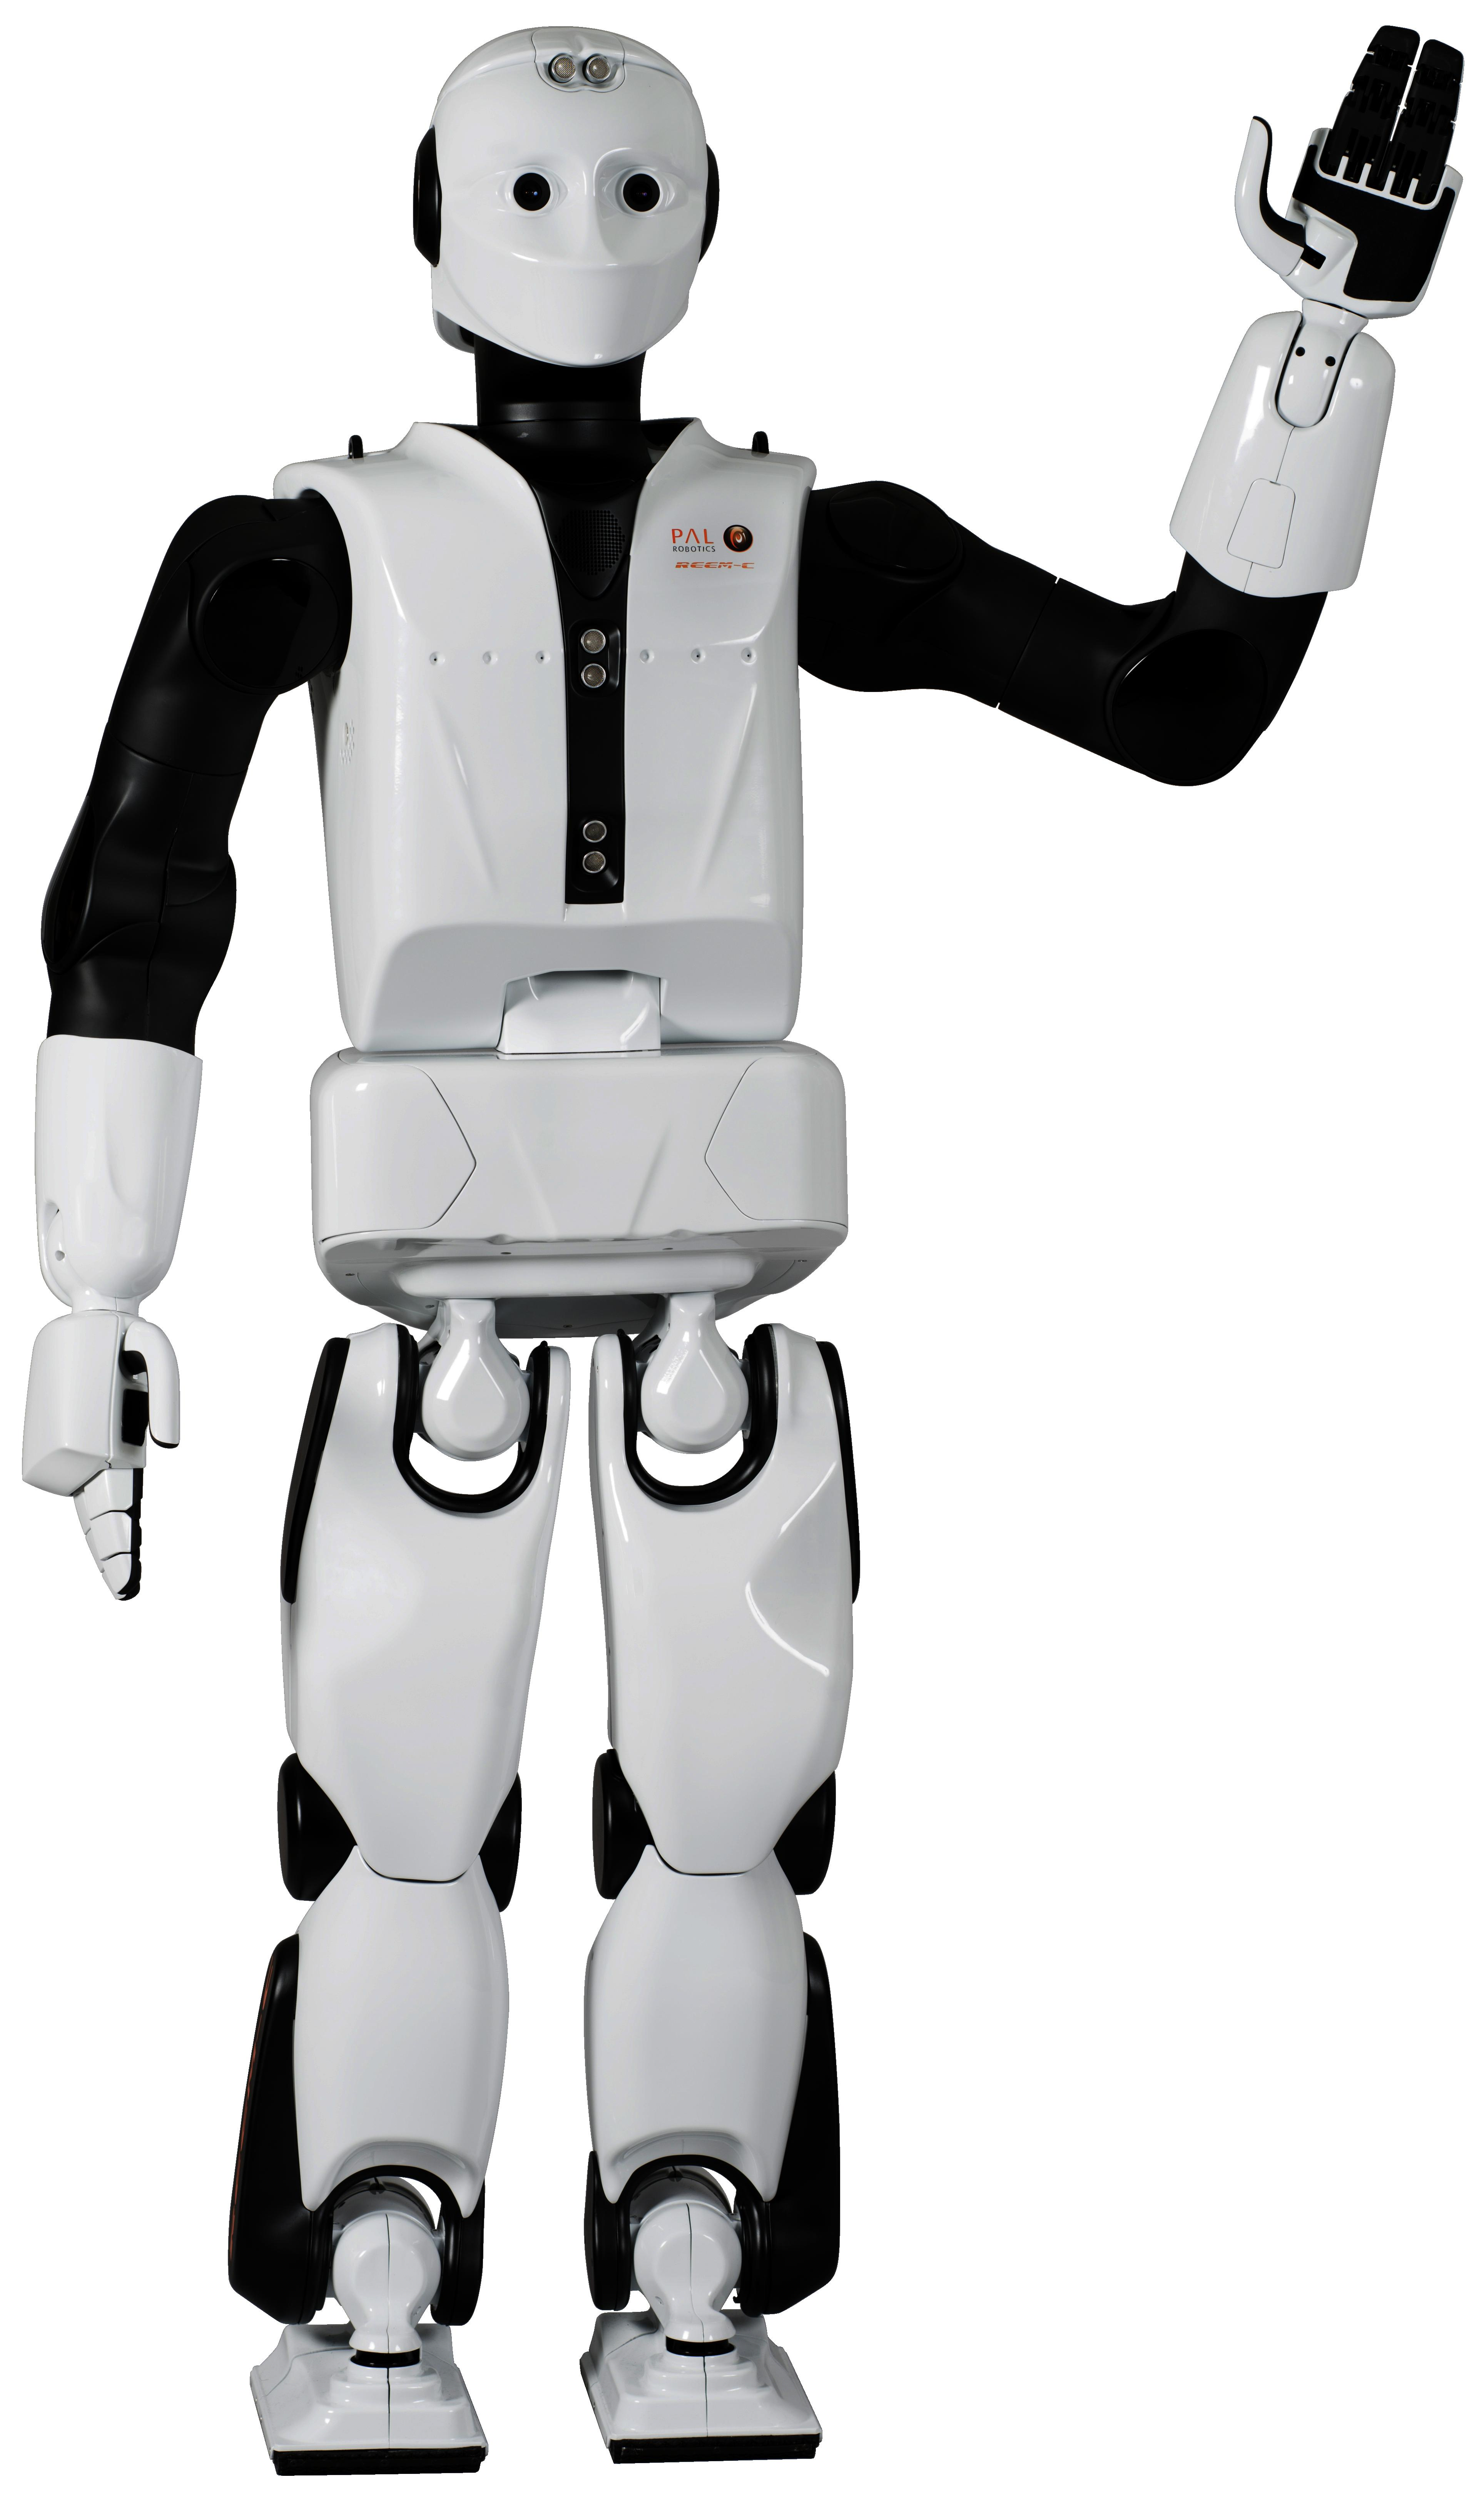
\includegraphics[width=0.18\textwidth]{../figures/reemc2.jpg}
    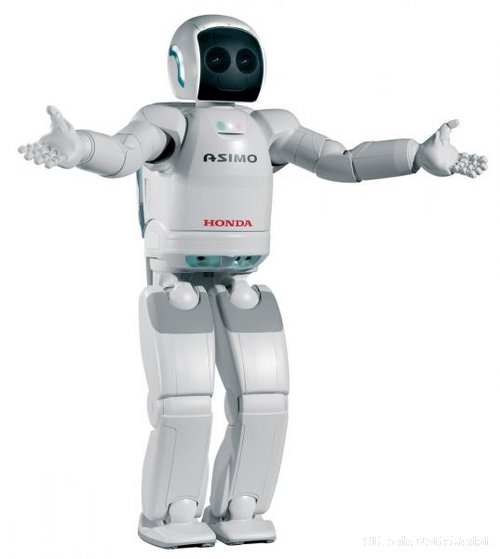
\includegraphics[width=0.23\textwidth]{../figures/asimo2.jpg}
    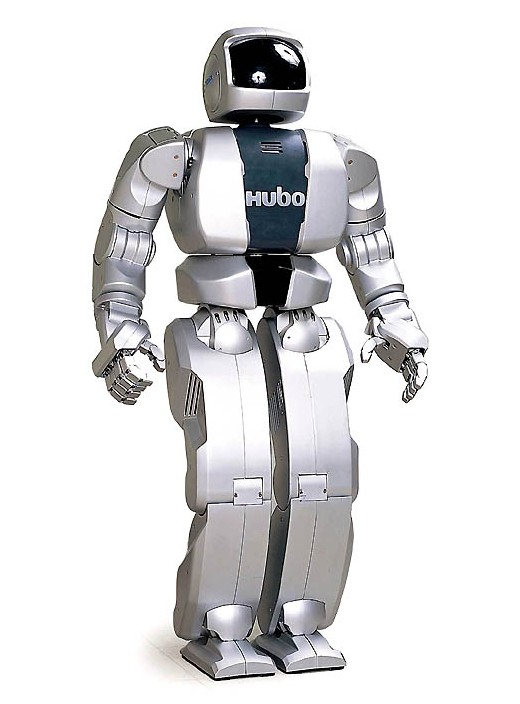
\includegraphics[width=0.23\textwidth]{../figures/hubo.jpg}
    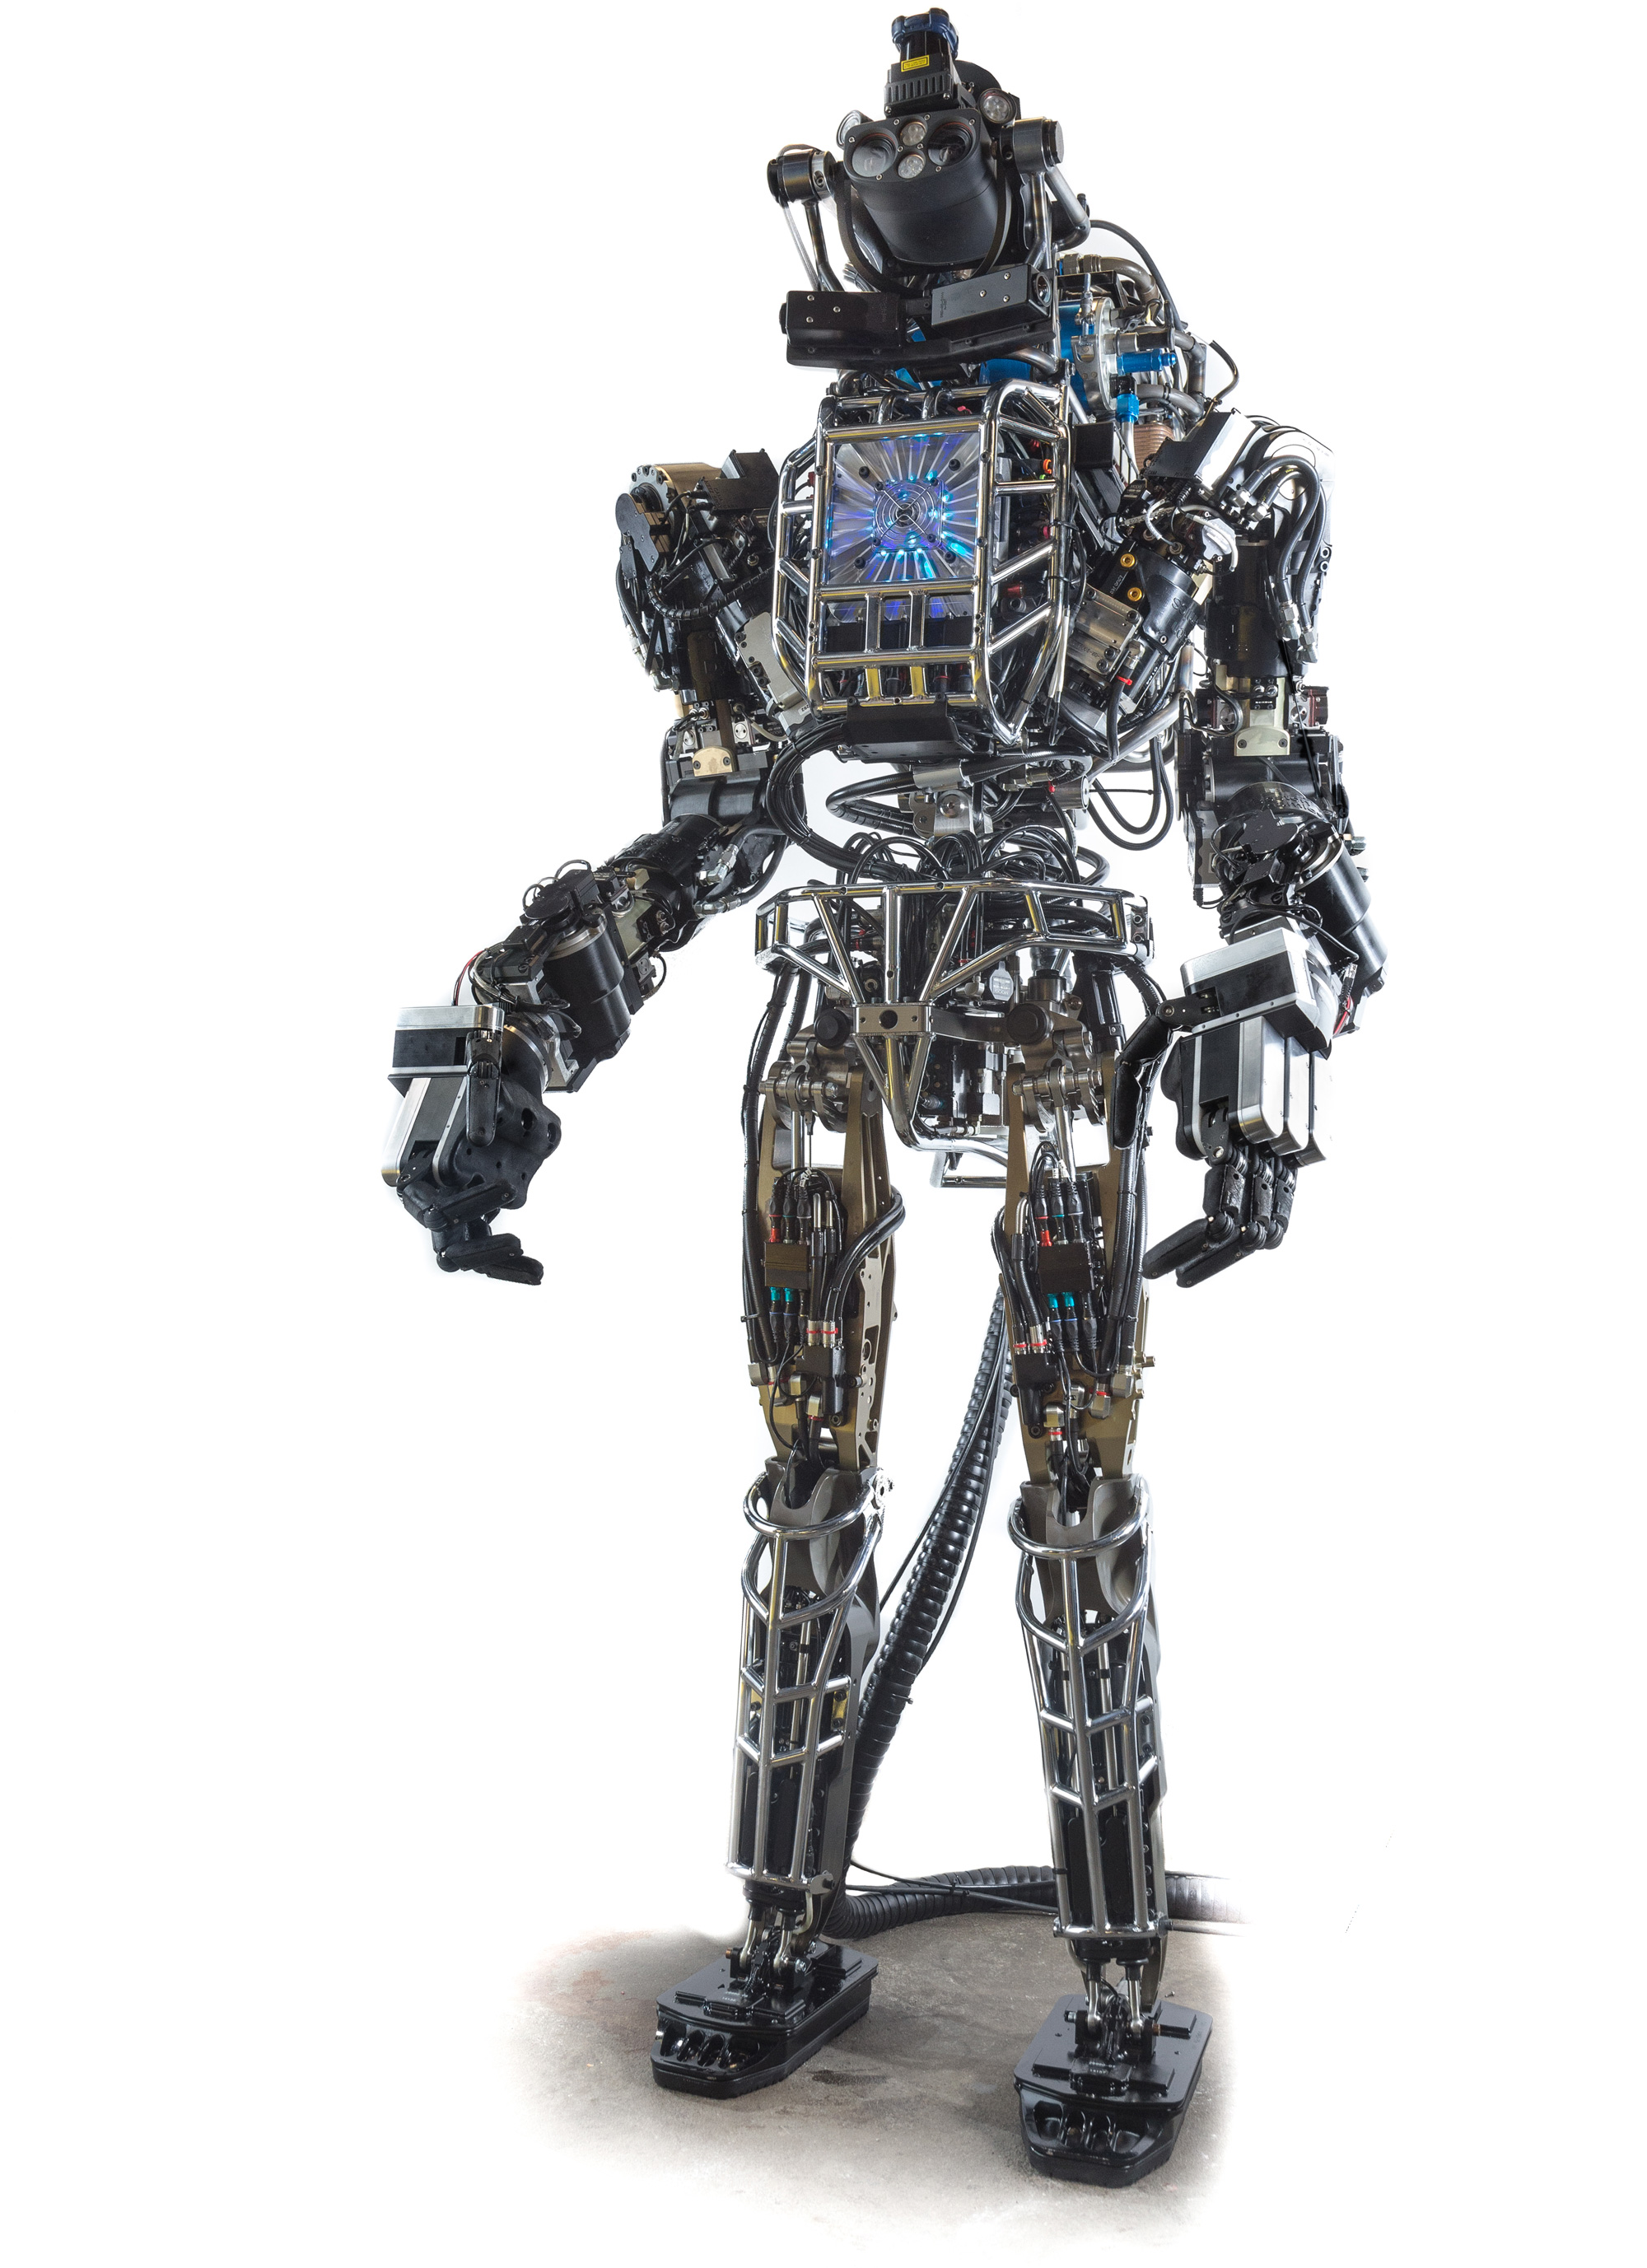
\includegraphics[width=0.23\textwidth]{../figures/atlas.jpg}
    \caption{State-of-the-art humanoid robots. From left: REEM-C, Asimo, Hubo, Atlas}
    \label{figclosestpointmesh}
\end{figure}
The dexterity and execution speed of humanoid robots thus encourage their integration into human environments. The idea of a robot accompanying a human in his daily life is becoming closer to practice. Complex tasks such as cleaning, ironing clothes or acting as a personal assistant are no longer futuristic visionary ideas, but already realizable at this time. 

What follows is the necessity of addressing safety issues, which emerge as a consequence of high execution velocities. Collisions with the robot environment as well as with the robot themselves have to be stringently avoided at all times. This becomes non-trivial especially with versatile humanoid robots, as they might easily collide with themselves, due to the redundant degrees of freedom (DOF) or the overlapping workspace of the attached manipulators (hand to hand collision). 

One way to handle collisions can be achieved by utilizing offline motion planners \cite{LaValle04planningalgorithms}. The complete scene is captured and an optimal solution without any collisions is planned. Once the trajectory is found, it is executed on the robot \cite{conf/iros/LiuDZ05}. In order to increase the speed of this planning step, especially with respect to avoiding obstacles, various optimization approaches are suggested. Rapidly-Exploring Random Trees (RRT) \cite{Lavalle98rapidly-exploringrandom} or Kinodynamic Motion Planning by Interior-Exterior Cell Exploration (KPIECE) \cite{644} are two methods, which are widely integrated in current motion planning libraries \cite{ompl}. Probabilistic Roadmaps (PRM) \cite{Kavraki96probabilisticroadmaps} are equally efficient, when the complete scene is known a priori. Probabilistic approaches \cite{Thrunprobabilisticalgorithms} are generally used to find an optimal solution. 

As the name \textit{offline} planner suggests, the trajectory planning and collision avoidance occur before the actual execution. Since the perception of the environment is still computational expensive, it is not surprising that those approaches are less efficient in dynamic environments. A fast-changing environment demands a highly reactive change of the current trajectory, still avoiding any collisions. \\
\textit{Reactive} collision avoidance algorithms try to overcome this issue. A first approach was based on repulsive forces emitted by the obstacles \cite{Khatib:86g}. Real time enabled collision avoidance based on repulsive forces have been broadly used on humanoid robots \cite{conf/humanoids/SugiuraGJG06} \cite{Xie98real-timecollision}  \cite{conf/iros/SetoKH05}. 
An enhanced development of this approach has been examined by calculating the closest point pairs between two collision objects and orient the repulsive force along the resulting directional vector \cite{conf/icra/DietrichWTAH11}. However, this implies a continuity of these calculated point pairs in order to avoid singularities and the resulting high velocities on the robot actuators \cite{escande:itro:2013}.

Since humanoid robots are highly over-actuated systems, their redundancy implies a null\-space optimization \cite{12020}, in which multiple goals can be achieved simultaneously. Within this, whole body motion control describes how to achieve a desired goal pose, utilizing all available joints. However, since multiple goal tasks can conflict with each other, priority levels are commonly used \cite{ROB:2555180}\cite{Sentis:06} and can be solved in a recursive hierarchical manner \cite{siciliano1991general}. We have therefore developed a method that ensures a collision avoidance on a high priority, but equally provides a sufficiently large nullspace to execute lower priority tasks. 
\newpage
\section{Goals of this thesis}
This work presents a complete solution for external as well as self-collision avoidance of humanoid robots. The presented implementation is based on the proposed algorithm in \cite{stasse-icra-08}. The collision avoidance is realized as an inequality constraint inside the Stack-of-Tasks (SoT) \cite{mansard:icar:09}, which serves as the base framework throughout this work. The SoT provides a highly efficient solver for hierarchical quadratic programming, which allows the execution of simultaneous goals in a whole body control manner. The algorithm in \cite{stasse-icra-08} restricts any movement along the directional vector between two closest points. In order to achieve a smooth trajectory of the closest point pair, we suggest a complete capsule decomposition as the robot's collision representation. The closest point pair is thus calculated between two capsules in order to ensure a smooth continuation in time.\\
This work is developed on two humanoid robots from PAL Robotics S.L., namely REEM-H and REEM-C. Since both robots are completely ROS based, the first goal is to integrate the SoT inside the ROS environment. 

As a summary, solutions for the following goals are presented:
\begin{itemize}\label{item:goals}
\item Integrate the SoT inside a ROS based environment to enable the execution on PAL Robotics humanoid robots
\item Assemble the robot collision model through a complete capsule decomposition to allow a smooth and continuous calculation of a closest point pair
\item Implement a collision avoidance task inside the SoT, utilizing the calculated point pair to ensure no self-collision and to enable support for external collision avoidance.
\end{itemize}

\section{Overview of this thesis}
Part \ref{part:introAndBackgroundTheory} of this work explains all the theoretical details, which are necessary for understanding the concepts implemented in this work. After this introduction, chapter \ref{chapter:soth} introduces the Stack-of-Tasks (SoT) from a theoretical point of view. We present background information about how to specify tasks based on equality and inequality constraints inside a quadratic program. Since the main objective of this thesis is the development of a collision avoidance task, we dedicate chapter \ref{chapter:collisionavoidance} to details on the implemented method. 

Implementation details and practical experiments, conducted on the robot are presented in part \ref{part:implementation}. We briefly introduce the implementation environment in chapter \ref{chapter:implenv}, where we describe ROS\_control as the main control framework, running on REEM-H and REEM-C. We further give information on how to integrate the SoT into a ROS based environment. Since the SoT comprises a complete framework, including the numerical solver, we describe the main functionalities, which are necessary for implementing a (self-)collision task. The main method, which is implemented to achieve a successful collision avoidance, has to be supplemented with additional tasks, e.g. joint limits. The instantiated tasks, which run on the robot to perform successful collision avoidance, are presented in chapter \ref{chapter:collisionavoidanceimpl}. In order to evaluate the implemented methods, various tests for all specified goals of chapter \ref{item:goals} are examined and analyzed in chapter \ref{chapter:experiments}. Finally, in chapter \ref{chapter:applications} we provide applications, which are successfully realized and give an outlook about further developments.